\chapter{Electricity and Magnetism}

\pagestyle{fancy}
\fancyhf{}
\fancyhead[OC]{\leftmark}
\fancyhead[EC]{\rightmark}
%\renewcommand{\footrulewidth}{1pt}
\cfoot{\thepage}

\section{Level 1 Problems and Solutions}
\begin{tcolorbox}
\textbf{1. Three point charges q, 2q and 8q are to be placed on a 9cm long straight line. Find the positions where the charges should be placed so that the potential energy of the system is minimum.}
\end{tcolorbox}
Solution:
\begin{figure}[h]
    \centering
    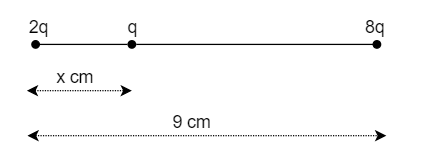
\includegraphics[scale = 0.8]{figures/Sandesh's Figures/threePtChar.png}
    % \caption{Conversion of soap bubble into spherical drop.}
    \label{fig3}
\end{figure}

 Since the potential energy is directly proportional to the product of charges and inversely proportional to the distance between them, we need to have a preliminary idea that the two greater charges should be placed as far as possible. In this case, they should be placed at two ends of a 9 cm line.\\
 Let, the charge q be placed at a distance x from 2q.
 Potential energy of the system is given as,
 \begin{equation}
     U = \cfrac{1}{4 \pi \epsilon_o} \bigg(\cfrac{2q \cdot q}{x} + \cfrac{2q \cdot 8q}{9} + \cfrac{q \cdot 8q}{9 - x} \bigg)
 \end{equation}
 For U to be minimum,
 \begin{align*}
 \cfrac{dU}{dx} &= 0\\
 or, \cfrac{2q^2}{4 \pi \epsilon_o}\bigg(\cfrac{dx^{-1}}{dx} + 0 + 4 \cdot \cfrac{d(9 - x)^{-1}}{dx}\bigg) &= 0\\
 or, - \cfrac{1}{x^2} + \bigg(\cfrac{2}{9 -x}\bigg)^2 &= 0 \\
 or, \cfrac{2}{9 -x} &= \cfrac{1}{x}\\
 or, 2x &= 9 - x \\
 \therefore x &= 3 cm
 \end{align*}
 Therefore, for the potential energy of the system to be minimum, the smallest charge q should be placed between 2q and 8q at a distance of 3 cm from 2q.
 \begin{tcolorbox}
\textbf{2. An electric dipole with dipole moment $\bm{p}$ is in a uniform electric field $\bm{E}$.\\
i. Find the operations of the dipole for which the torque on the dipole is zero.\\
ii. Which of the operations in part (i) is stable, and which is unstable?\\
iii. Show that for the stable orientation in part (ii), the dipole's own electric field tends to oppose the external field.}
\end{tcolorbox}
Solution:\\
Torque on a dipole ($\tau$) = $\bm{p} \times \bm{E}$ = pE $sin \theta$\\
i. So torque will be zero for $\theta$ = n$\pi$, where n = 0,1,2,3..., i.e. torque will be zero if the direction of dipole moment is along $\bm{E}$, or if it is exactly opposite to $\bm{E}$.
\begin{figure}[h]
    \centering
    \begin{subfigure}[b]{0.45\textwidth}
    \centering
    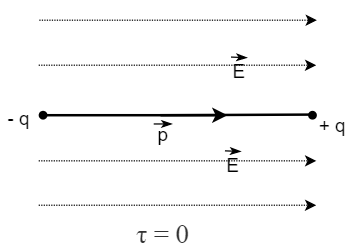
\includegraphics[scale = 0.6]{figures/Sandesh's Figures/dipoles1.png}
     \caption{$\bm{p}$ in the direction of $\bm{E}$.}
     \label{dp1}
    \end{subfigure}
    \hfill
     \begin{subfigure}[b]{0.45\textwidth}
     \centering
    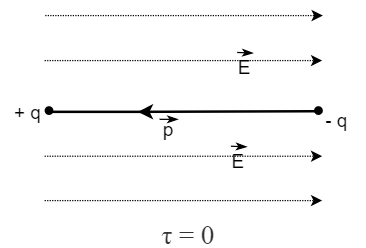
\includegraphics[scale = 0.6]{figures/Sandesh's Figures/dipoles2.png}
     \caption{$\bm{p}$ opposite to $\bm{E}$.}
     \label{dp2}
    \end{subfigure}
    
    \caption{Orientations of the dipole for which the torque is zero.}
    \label{dipoles}
\end{figure}
\\ii. Consider the orientation in \ref{dp1}
\begin{figure}[h]
    \centering
    \begin{subfigure}[b]{0.45\textwidth}
    \centering
    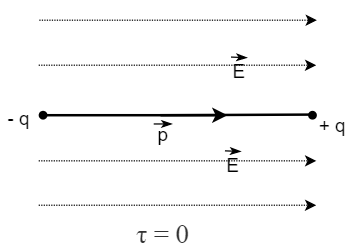
\includegraphics[scale = 0.6]{figures/Sandesh's Figures/dipoles1.png}
     \caption{$\bm{p}$ in the direction of $\bm{E}$.}
     \label{dp}
    \end{subfigure}
    \hfill
     \begin{subfigure}[b]{0.45\textwidth}
     \centering
    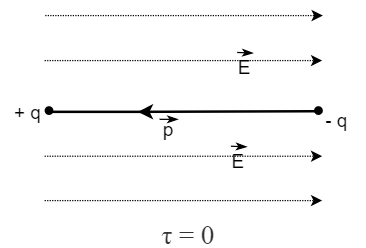
\includegraphics[scale = 0.6]{figures/Sandesh's Figures/dipoles2.png}
     \caption{$\bm{p}$ opposite to $\bm{E}$.}
     \label{dp}
    \end{subfigure}
    \caption{Orientations of the dipole for which the torque is zero.}
    \label{dipoles}
\end{figure}

If we slightly shift the zero torque orientation in \ref{dp1} either up or down as shown in \ref{}, then the torque will be produced in such a way that it rotates the dipole to acquire the initial configuration. So, it is stable.\\

Now, consider the orientation in \ref{dp2}. \\
\begin{figure}[h]
    \centering
    \begin{subfigure}[b]{0.45\textwidth}
    \centering
    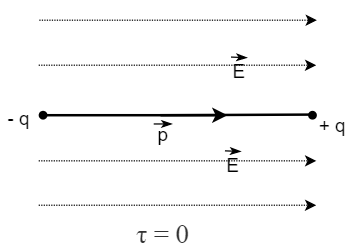
\includegraphics[scale = 0.6]{figures/Sandesh's Figures/dipoles1.png}
     \caption{$\bm{p}$ in the direction of $\bm{E}$.}
     \label{dp}
    \end{subfigure}
    \hfill
     \begin{subfigure}[b]{0.45\textwidth}
     \centering
    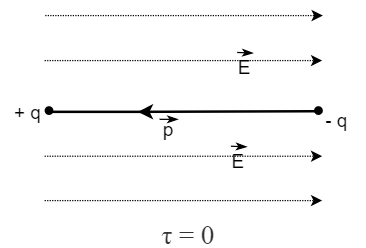
\includegraphics[scale = 0.6]{figures/Sandesh's Figures/dipoles2.png}
     \caption{$\bm{p}$ opposite to $\bm{E}$.}
     \label{dp}
    \end{subfigure}
     \caption{Orientations of the dipole for which the torque is zero.}
    \label{dipoles}
\end{figure}
In this case a slight shifting of orientation will rotate the dipole further away from the equilibrium position. So, it is unstable.

iii. Since the electric field of the dipole is from +q to -q we can wasily see from above figures \ref{}, \ref{} and \ref{}, that the dipole's own electric field tends to oppose the external field.



\newpage
\section{Level 2 Problems and Solutions}
\begin{tcolorbox}
\textbf{1. If the radius and surface tension of a spherical soap bubble be r and T respectively, calculate the charge required to double its radius.} 
\end{tcolorbox}
 Solution:
\begin{figure}[h]
    \centering
    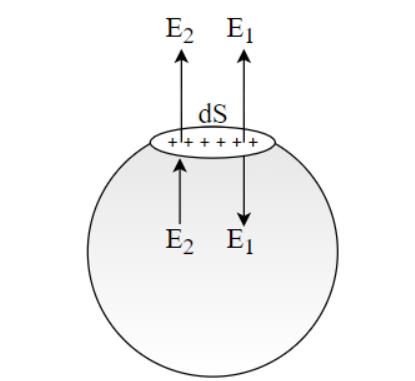
\includegraphics[scale = 0.5]{figures/Sandesh's Figures/fig1.png}
    \caption{
 Electric fields due to dS and the remaining area of the soap bubble }
    \label{fig1}
\end{figure}

 Irrespective of the nature of concentrated charges in the soap bubble (either positive or negative), the electrostatic repulsion between them causes the soap bubble to expand.\\

Consider a soap bubble with uniform charge density $\sigma$ distributed over the surface. Now, consider dS, a small area of the spherical surface, which acts as a thin sheet of charge. The electric field, $E_1$, due to this thin sheet of charge on its either direction is given as 
\begin{equation}\label{eq1}
    E_1 = \cfrac{\sigma}{2\epsilon_o}
\end{equation}
Now,\\
$E_2$ be the electric field due to remaining portion of the spherical surface (i.e. excluding dS). The direction of $E_2$ is as shown in the figure because of the spherical symmetry of the charge distribution. Inside the soap bubble, electric field is zero. So, $E_1$ and $E_2$ should be equal and opposite. 
\begin{equation}\label{eq2}
    E_2 = E_1 = \cfrac{\sigma}{2\epsilon_o}
\end{equation}
The force on the surface dS, 
\begin{equation}\label{eq3}
    dF = \sigma . dS . E_2
\end{equation}
where $\sigma . dS$ is the small amount of charge on the surface dS.\\
From equation \ref{eq2} and \ref{eq3}, we get
\begin{equation}\label{eq4}
    P_{elec} = \cfrac{\sigma^2}{2\epsilon_o}
\end{equation}
The electric pressure given by \ref{eq4} acts from inside to outside the soap bubble and expands it.\\

\begin{wrapfigure}{r}{2in}
     \centering 
     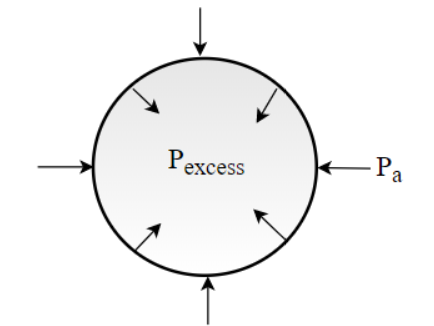
\includegraphics[scale = 0.5]{figures/Sandesh's Figures/fig2.png}
     \caption{Point $P_1$ located outside the spherical volume, that is, r $>$ R. }
     \label{fig5}
 \end{wrapfigure}
Before the application of charge, initial pressure acting inside the soap bubble is 
\begin{equation}\label{eq5}
    P_{in} = P_a + \cfrac{4T}{r}
\end{equation}
where,\\
$P_a$ = Atmospheric pressure, and
$\dfrac{4T}{r}$ = Excess pressure in a soap bubble of radius r.Note that the excess pressure is due to surface tension which intends to reduce the size of the bubble.\\
When the soap bubble is charged, it experiences outward pressure as discussed by equation \ref{eq4}. So with reference to \ref{eq4} and \ref{eq5}, the final pressure acting inside the soap bubble is reduced and given as 

\begin{equation}
    P_f = P_a + \cfrac{4T}{R} - \cfrac{\sigma^2}{2\epsilon_o}
\end{equation}
where R is the final radius after expansion. It is important to realize that this expansion is slow and isothermal so that we can use  Boyle's law. Therefore,
\begin{equation}
    P_{in}V_{in} = P_f V_f
\end{equation}
\begin{align*}
\text{or, }\bigg(P_a + \cfrac{4T}{r}\bigg) . \cfrac{4}{3} \pi r^3 &= \bigg(P_a + \cfrac{4T}{R} - \cfrac{\sigma^2}{2\epsilon_o}\bigg) . \cfrac{4}{3} \pi R^3\\
\text{or, } P_a (R^3 - r^3) + 4T (R^2 - r^2) &= \cfrac{q^2}{32\epsilon_o\pi^2R} \hspace{8pt} \bigg[\because \cfrac{\sigma^2}{2\epsilon_o} = \cfrac{q^2}{32\epsilon_o\pi^2R^4}\bigg]
\end{align*} 
Given, R = 2r. So,
\begin{align*}
P_a (8r^3 - r^3) + 4T (4r^2 - r^2) &= \cfrac{q^2}{32\epsilon_o\pi^2 2r}\\
\text{or, }  7P_ar^3 + 12Tr^2 &= \cfrac{q^2}{64\epsilon_o\pi^2r}\\
\text{or, }q^2 &= 64 \pi^2 (7P_a\epsilon_or^4 + 12 T\epsilon_or^3)
\end{align*}
$\therefore q = 8\pi r \sqrt{\epsilon_or(7P_ar + 12T)}$ is the amount of charge required to double the radius of the spherical soap bubble.

\pagebreak
\begin{tcolorbox}
\textbf{
2. A soap bubble 10 cm in radius with a wall thickness of $3.3 \times 10^{-6}$ cm is charged to a potential of 100 V. The bubble bursts and falls as a spherical drop. Estimate the potential of the drop. \begin {FlushRight}- NePhO 2018 \end{FlushRight}}
\end{tcolorbox}
Solution:\\

\begin{figure}[h]
    \centering
    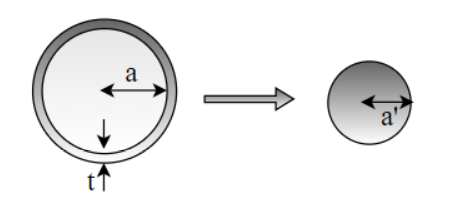
\includegraphics[scale = 0.8]{figures/Sandesh's Figures/fig3.png}
    \caption{Conversion of soap bubble into spherical drop.}
    \label{fig3}
\end{figure}

We solve this problem by using the concept of spherical capacitors.\\
Let Q be the charge supplied to the soap bubble of radius a and thickness t. If we draw a spherical Gaussian surface outside the soap bubble at any distance r from its center ($r > a$),then Gauss's law gives,
\begin{align*}
E \cdot A &= \cfrac{Q}{\epsilon_o}\\
\text{or, }E \cdot 4\pi r^2 &= \cfrac{Q}{\epsilon_o}
\end{align*}
$\therefore E = \cfrac{Q}{4\pi \epsilon_o r^2}$ is the electric field normal to the Gaussian surface.\\
Since we know that the electric field is the negative gradient of potential \bigg(i.e. $E = - \cfrac{dV}{dr}$\bigg), we can find the potential of the soap bubble by integrating -E with respect to r from r = $\infty$ to r = a.
Therefore, 
\begin{align*}
 V_a - V_{\infty} &= \int_{\infty}^a E\cdot dr\\
\text{or, }  V_a &= - \cfrac{Q}{4\pi \epsilon_o a} \int_{\infty}^a \cfrac{dr}{r^2}\\
\text{or, } V_a &= \cfrac{Q}{4\pi\epsilon_o a}
\end{align*}
Therefore, the soap bubble of radius a and charged to potential $V_a$ should carry the charge, 
\begin{equation}\label{eq8}
    Q = 4\pi \epsilon_o a V_a
\end{equation}
When the bubble bursts, volume of the new drop formed should be equal to the volume of liquid contained in the bubble. If a' be the radius of the new drop then,
\begin{align*}
 \cfrac{4}{3} \pi (a + t)^3 - \cfrac{4}{3} \pi a^3 = \cfrac{4}{3} \pi a'^{3}\\
\text{or, } a^3 + 3a^2t + 3at^2 + t^3 - a^3 = a'^{3}
\end{align*}
Since t is very small, the terms containing its higher powers are further smaller and can be neglected. So, 
\[ 3a^2t = a'^{3}\]
\begin{equation}\label{eq9}
    \therefore a' = (3a^2t)^{\tfrac{1}{3}}
\end{equation}  

\bigg[Or, we could have simply done 4$\pi a^2 t = \cfrac{4}{3} \pi a'^{3}$, with the logic that volume is surface area (4$\pi a^2)$ times thickness (t)\bigg]\\

Since charge is conserved, the newly formed drop will act as a spherical capacitor of radius a' having charge Q =$ 4\pi \epsilon_o a V_a$ (from \ref{eq8}) uniformly distributed over its surface. As the drop of soap solution is a conductor, no charge rests inside. \\
Capacitance of the drop, \begin{equation}\label{eq10}
    C = 4 \pi \epsilon_o a'
\end{equation}
Hence, the potential of the drop, \[ V = \cfrac{Q}{C}\]
Solving by using the expression for Q, C and a' from \ref{eq8}, \ref{eq10} and \ref{eq9} respectively, we get \[ V = \cfrac{a}{(3a^2t)^{\tfrac{1}{3}}} \hspace{2pt}V_a \]

Putting a = 10 cm = 0.1 m, t= $3.3 \times 10^{-8}$ m, and $V_a = 100$ V, we obtain the potential of the drop as 10 kV.\\
\pagebreak

\begin{tcolorbox}
\textbf{3. Calculate the amount of work needed to assemble a system at which -e charges are placed at each corner of a cube of length d and +2e at its center. }
\end{tcolorbox}
Solution:\\

\begin{figure}[h]
    \centering
    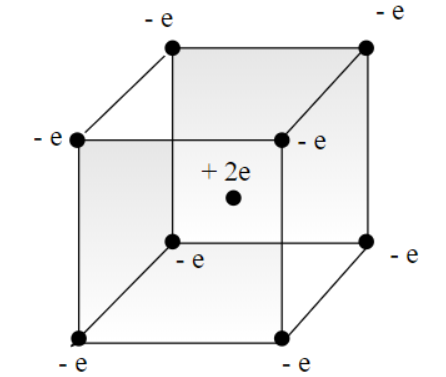
\includegraphics[scale = 0.59]{figures/Sandesh's Figures/fig4.png}
    \caption{System of eight -e and one +2e charges arranged on a cube.}
    \label{fig4}
\end{figure}


Initially assume that the charges are separated at infinite distance from one another such that the potential energy of the system is zero.
\\
When the charges are then assembled as shown in figure \ref{fig4}, the amount of work done is equal to the final potential energy of the system. \\
Here, number of charges (n) = 9 \\
So, the number of pairs that can be formed is given by \[\cfrac{n(n-1)}{2} = 36\]
On analyzing, we get
\begin{enumerate}[label=\roman*)]
    \item 12 pairs of -e and -e separated by d (i.e adjacent ones)
    \item 12 pairs of -e and -e separated by $\sqrt{2}$d (i.e across the digonals of each face)
    \item 4 pairs of -e and e separated by $\sqrt{3}$d (i.e across the diagonals of the cube)
    \item 8 pairs of -e and +2e separated by $\cfrac{\sqrt{3}}{2}$d (i.e from each corner to the center of the cube)
\end{enumerate} 
Therefore the electric potential energy of the assembled system is given by \[ U = 12\cdot \cfrac{(-e)(-e)}{4\pi\epsilon_o d} + 12\cdot \cfrac{(-e)(-e)}{4\pi\epsilon_o \sqrt{2}d} + 4\cdot \cfrac{(-e)(-e)}{4\pi\epsilon_o\sqrt{3}d} + 8\cdot \cfrac{(-e)(+2e)}{4\pi\epsilon_o \cfrac{\sqrt{3}}{2}d} \]
On solving we get an expression for U which the required work done. $$U = \cfrac{1.08e^2}{\pi\epsilon_od}$$


\begin{tcolorbox}
\textbf{4. Calculate the potential energy of a charge Q uniformly distributed throughout the sphere of radius R.}
\end{tcolorbox}
Solution:
This problem can be solved by calculating the amount of work done in assembling a sphere of total charge Q uniformly distributed throughout its volume.\\
Let $\rho$ be the volume charge density.\\
In the process of assembling a sphere, let, at any instant, the sphere has radius r and charge q.\\
\[ q = \cfrac{4}{3}\pi \rho^3\]
Since charge distribution is uniform throughout the volume,
\begin{equation*}
\begin{split}
\cfrac{q}{Q} &= \cfrac{\cfrac{4}{3}\pi \rho r^3}{\cfrac{4}{3}\pi \rho R^3}\\
\vspace{3pt}
\therefore q &= \cfrac{Qr^3}{R^3}
\end{split}
\end{equation*} 
If we add a spherical shell of thickness dr to the sphere of radius r, then the amount of charge added,
\begin{equation*}
\begin{split}
   dq &= \rho \cdot 4\pi r^2 \cdot dr \\
   &= \cfrac{Q}{\cfrac{4}{3}\pi R^3} \times 4 \pi r^2 dr\\
   \vspace{3pt}
   \therefore dq &= \cfrac{3Qr^2}{R^3}\hspace{3pt} dr
   \end{split}
\end{equation*}
So, the small amount of work done in assembling dq to a sphere of radius r, and carrying charge q,\\\\
\begin{center}
dW = V$\cdot$ dq \hspace{5mm} \big [$\because$ Potential = Work Done / Charge]
\end{center}
where,
$V = \cfrac{1}{4\pi\epsilon_o}\cfrac{q}{r}$ is the potential of a sphere of radius r.
\\
The total work done in assembling all the shells of charges to form a complete sphere of radius R and charge Q is 
\[ W = \int _0^R V\cdot dq = \int_0^R \cfrac{1}{4 \pi \epsilon_o}\cdot \cfrac{q}{r}\cdot \cfrac{3Qr^2}{R^3}\cdot dr \]
\begin{equation}\label{eq11}
    \therefore W = \cfrac{3Q^2}{20\pi\epsilon_o R}
\end{equation}
The work done is equal to the potential energy. So, equation \ref{eq11}, gives the expression for potential energy of a charge Q uniformly distributed throughout the sphere. 

\begin{tcolorbox}
\textbf{5. Calculate the electric potential at\\
i. r $>$ R\\
ii. r $=$ R\\
iii. r $<$ R\\
due to a uniformly charged non-conducting sphere of radius R containing charge Q.}
\end{tcolorbox}
Solution:\\
Solving i. and ii. should be a piece of cake, whereas iii. requires a little effort.\vspace{2pt}
\\In a non-conducting sphere, charge is uniformly distributed throughout the volume with density, \[\rho = \cfrac{Q}{\dfrac{4}{3}\pi R^3}\]
The potential at infinity is zero.
\vspace{3pt}\\
i. \underline{Outside the spherical volume (r $>$ R).}
\vspace{5pt}

\begin{wrapfigure}{r}{2in}
     \centering 
     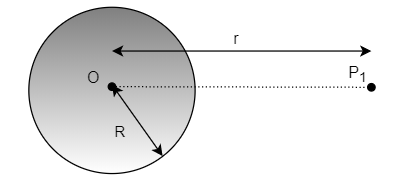
\includegraphics[scale = 0.6]{figures/Sandesh's Figures/fig5.png}
     \caption{Point $P_1$ located outside the spherical volume, that is, r $>$ R. }
     \label{fig5}
 \end{wrapfigure}
Consider a point P outside the spherical volume located at a distance r from the center.
Magnitude of electric field at $P_1$,
\[E_1 = \cfrac{1}{4 \pi \epsilon_o}\cdot \cfrac{Q}{r^2}\]
Electrostatic potential at $P_1$,
\begin{align*}
V_1 = -\int_\infty^r E_1 \cdot dr &= - \int_\infty^r \cfrac{1}{4 \pi \epsilon_o}\cdot \cfrac{Q}{r^2} \cdot dr
 \therefore V_1 &= \cfrac{1}{4 \pi \epsilon_o}\cdot \cfrac{Q}{r} 
\end{align*}
This is same as if the charge were placed at the center. Thus, for external points the spherical charge behaves s if the whole charge were concentrated at the center of the spherical charge distribution.
\vspace{4pt}\\
\begin{wrapfigure}{r}{1.8in}
     \centering 
     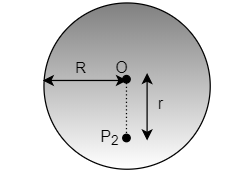
\includegraphics[scale = 0.7]{figures/Sandesh's Figures/fig6.png}
     \caption{Point $P_2$ located inside the spherical volume, that is, r $<$ R. }
     \label{fig5}
 \end{wrapfigure}
ii. \underline{At the surface (r = R)}
\vspace{5pt}
\\ Following a similar approach as i.,we would integrate from $\infty$ to R to get the required potential, 
\[ V_R = \cfrac{1}{4 \pi \epsilon_o}\cdot \cfrac{Q}{R} \]

iii. \underline{Inside the spherical volume (r $<$ R)}
\vspace{5pt}
\\ This is the major crux, and is the reason why the entire problem is included here in the first place. You would see how simply it can be solved.
\vspace{2pt}
\\
Consider a point $P_2$ inside the spherical charge at a distance r from the center O. To find the potential at $P_2$, we have to come from infinity to $P_2$
passing through regions having two different expressions for electric field.\\

 At r $>$ R,
\[  E_1 = \cfrac{1}{4 \pi \epsilon_o}\cdot \cfrac{Q}{r^2}\]

At r $<$ R,
\[ E_2 = \cfrac{1}{4 \pi \epsilon_o}\cdot \cfrac{Qr}{R^3}\]
Expression for $E_2$ can simply be calculated using Gauss's law, where $Q_{enclosed} = \dfrac{Qr^3}{R^3}$, resulting from uniform volume charge distribution.
\\
Now,
\\
Required potential at $P_2$ is given as,
\begin{equation*}
\begin{split}
V_2 &= -\int_\infty^r E \cdot dr\\
    &= - \bigg[\int_\infty^R E_1 \cdot dr  +  \int_R ^r E_1 \cdot dr\bigg]\\ 
    &= - \bigg[\int_\infty^R \cfrac{1}{4 \pi \epsilon_o}\cdot \cfrac{Q}{r^2} \cdot dr + \int_R ^r\cfrac{1}{4 \pi \epsilon_o}\cdot \cfrac{Qr}{R^3} \cdot dr \bigg]\\
    &= -\cfrac{Q}{4 \pi \epsilon_o} \bigg[ \bigg(-\cfrac{1}{r}\bigg)_\infty^R + \cfrac{1}{R^3}\bigg(-\cfrac{r^2}{2}\bigg)_R^r \bigg]\\
    &= -\cfrac{Q}{4 \pi \epsilon_o} \bigg[-\cfrac{1}{R} + \cfrac{r^2}{2R^3} - \cfrac{1}{2R} \bigg]\\
    &= -\cfrac{Q}{4 \pi \epsilon_o} \bigg[\cfrac{r^2}{2R^3} - \cfrac{3}{2R} \bigg]\\
    &= \cfrac{Q}{4 \pi \epsilon_o} \bigg[\cfrac{3R^2 - r^2}{2R^3}\bigg]\\
\end{split}
\end{equation*} 
You can use the similar approach to find the gravitational potential of a planet at r $<$ R. See I.E. Irodov 1.214 and give it a try. You will be pleased. \\

\newpage
\begin{tcolorbox}
\textbf{6. A thin wire ring of radius r has an electric charge q. What will be the increment of the force stretching the wire if a point charge $q_o$ is placed at the ring's center?}
\end{tcolorbox}
Solution:
\begin{wrapfigure}{r}{2.7in}
     \centering 
     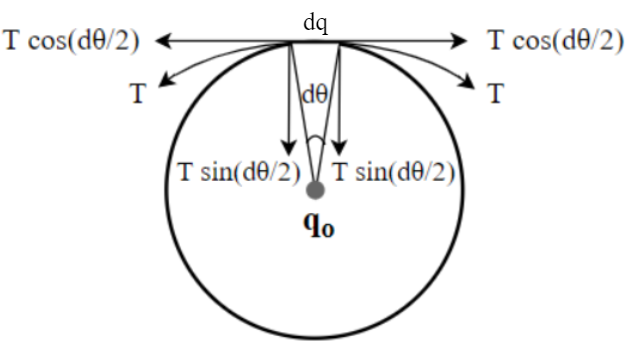
\includegraphics[scale = 0.46]{figures/Sandesh's Figures/tnsnrng.png}
     \caption{Point $P_2$ located inside the spherical volume, that is, r $<$ R. }
     \label{tnsrng}
 \end{wrapfigure}
When the charge $q_o$ is placed at the center of the ring then tension develops along the wire because of electrostatic force, which causes it to stretch.\\
Let us consider a small segment of the ring which subtends $d\theta$ at the center and contains charge dq.\\
Here,
\begin{align}
    dq &= \cfrac{q}{2 \pi r}\cdot r d\theta \nonumber\\
    \therefore dq &= \cfrac{q}{2 \pi} \cdot d\theta
\end{align} 

So, electrostatic force on dq, 
\begin{align}
    dF_e &= \cfrac{1}{4 \pi \epsilon_o} \hspace{5pt} \cfrac{q_o\cdot \cfrac{q}{2 \pi}\cdot d\theta}{r^2}\nonumber\\
    &= \cfrac{qq_o}{8\pi^2\epsilon_or^2}\hspace{5pt}d\theta \label{eq14}
\end{align}
From figure \ref{tnsrng}, we can see that the horizontal forces due to tension cancel out, and the vertical tension forces are given as,
\begin{align}
    dF_t &= T sin\cfrac{d\theta}{2} + T sin\cfrac{d\theta}{2}\nonumber\\
    &= 2T sin\cfrac{d\theta}{2}\nonumber\\
    &= Td\theta \label{eq15}
\end{align}
\begin{center}
$\big(\because$ for small angles, $\sin d\theta/2 \to d\theta/2.\big)$ \\
\end{center}
\vspace{5pt}
Here $dF_e$ and $dF_t$ are equal and opposite. So, equating equations \ref{eq14} and \ref{eq15} we obtain the required expression for the force.
\begin{align*}
    T\cdot d\theta &= \cfrac{qq_o}{8\pi^2\epsilon_or^2}\hspace{5pt}d\theta\\
    \therefore T &= \cfrac{qq_o}{8\pi^2\epsilon_or^2}
\end{align*}
\textbf{Note:} This approach is really important in solving several problems about ropes, strings or rings involving tension. Check out the following problem of Mechanics.
\pagebreak
\begin{tcolorbox}[colback=white]
\textbf{Q. A pole wraps at an angle $\theta$ around a pole. You grab one end and pull with tension T$_o$. The other end is attached to a large object, say, a boat. If the coefficient of static friction between the rope and the pole is $\mu$, what is the largest force the rope can exert on the boat, if the rope is not to slip around the pole?}\\
Solution:
\begin{wrapfigure}{l}{2.7in}
     \centering 
     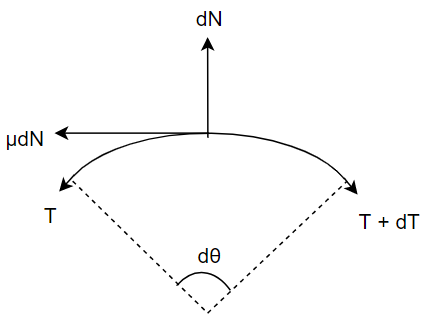
\includegraphics[width = 3.9cm,scale = 0.45]{figures/Sandesh's Figures/rppl.png}
     \caption{Tension, normal and frictional forces on a small segment of a rope wrapped around the pole. }
     \label{rppl}
 \end{wrapfigure}
 Since the rope is wrapped around the frictional surface(pole), and is pulled from one end, tension varies over the length. Consider small piece of rope that subtends an angle $d\theta$. Let the tension at  one end of this piece be T, which sightly varies(by dT) at the other end. The pole exerts a small outward normal force dN. To avoid slipping, friction should act in the direction of lesser tension.
 
Balancing forces in X-direction,
\begin{align} \label{eq16}
  T \cos\cfrac{d\theta}{2} + \mu dN &= (T + dT) \cos\cfrac{d\theta}{2}\nonumber\\
  \therefore \mu dN &= dT   
\end{align}
Balancing forces in Y-direction,
\begin{equation*} 
  dN = (T + dT) sin\cfrac{d\theta}{2} + T sin\cfrac{d\theta}{2}
\end{equation*}
\begin{equation}\label{eq17}
     \therefore \mu dN = dT
\end{equation}
Dividing \ref{eq16} by \ref{eq17} and integrating from T$_o$ to T and 0 to $\theta$ we get,
\[ T = T_o e^{\mu \theta}\]
which is the required expression for the largest force.
\end{tcolorbox}
\newpage
\begin{tcolorbox}
\textbf{7. There is a spherical cavity inside a ball charged uniformly with volume density $\rho$. The center of cavity is displaced with respect to the center of the ball by $\bm{a}$. Find the field strength $\bm{E}$ inside the cavity, assuming the permittivity equal to unity.}
\end{tcolorbox}
Solution:
\begin{wrapfigure}{r}{0.5\textwidth}
     \centering 
     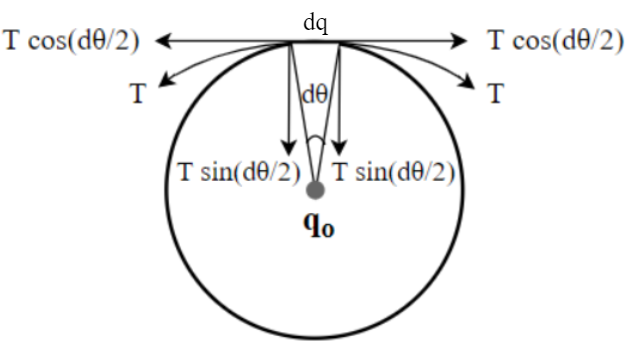
\includegraphics[scale = 0.46]{figures/Sandesh's Figures/tnsnrng.png}
     \caption{Point $P_2$ located inside the spherical volume, that is, r $<$ R. }
     \label{tnsrng}
 \end{wrapfigure}
 Let O and Q be the center of the ball and the spherical cavity respectively.\\
 We know,\\
 for a sphere with uniqform volume charge   density, electric field at any point inside is given by
 \begin{align}
     E &= \cfrac{1}{4 \pi \epsilon_o}\cdot \cfrac{qr}{R^3}\hspace{5pt} \hat{\textbf{r}} \nonumber \\
     &= \cfrac{q}{\cfrac{4}{3}\pi R^3} \cdot \cfrac{r}{3 \epsilon_o} \hspace{5pt}\hat{\textbf{r}} \nonumber \\
     &= \cfrac{\rho}{3 \epsilon_o} \hspace{5pt}\bm{\textbf{r}} \label{eq18}
 \end{align}
 \[ \bigg[\because Unit\hspace{4pt}vector (\hat{\textbf{r}}) = \cfrac{Vector (\bm{\textbf{r}})}{Magnitude (r)} \hspace{3pt}\bigg]\]
 \\
 \vfill
Now, let P be the any point inside the spherical cavity such that $\bm{OP}$ = $\bm{r_1}$ and $\bm{QP}$ = $\bm{r_2}$.
\vspace{3pt}
\\
Had there not been a cavity, then, with reference to equation \ref{eq18}, the electric field at P due to whole sphere would be, 

\begin{equation}
    E_1 = \cfrac{\rho}{3 \epsilon_o}\hspace{3pt} \bm{r_1}
\end{equation}
Similarly, had there been material on the cavity, the electric field at P only due to material of the cavity would be 
\begin{equation}
    E_2 = \cfrac{\rho}{3 \epsilon_o}\hspace{3pt} \bm{r_2}
\end{equation}
Since there is a cavity we need to subtract the effect due to material of the cavity $(\bm{E_2})$ from that of the entire sphere $(\bm{E_1})$ to obtain the electric field at point P in the cavity $(\bm{E})$. So,
\vfill
\begin{align*}
    \bm{E} &= \bm{E_1} - \bm{E_2} \\
            &= \cfrac{\rho}{3 \epsilon_o}\hspace{3pt} \bm{r_1} - \cfrac{\rho}{3 \epsilon_o}\hspace{3pt} \bm{r_2} \\
            &= \cfrac{\rho}{3 \epsilon_o} (\bm{r_1} -\bm{r_2})\\
            &= \cfrac{\rho}{3 \epsilon_o} \hspace{3pt}\bm{a}
\end{align*}
\vfill
Since the expression is independent of $\bm{r_1}$ and $\bm{r_2}$ we can say that the electric field inside the cavity is uniform. 

\newpage
\begin{tcolorbox}
\textbf{8. Two thin rods of length L lie along the x-axis, one between x = a/2 and x = a/2 + L, and the other between x = -a/2 and x = -a/2 - L. Each rod has positive charge Q distributed uniformly along its length.\\
i. Calculate the electric field produced by the second rod at points along the positive x-axis.\\
ii. Calculate the magnitude of the force one rod exerts on the another.\\
iii. Reduce the result of part ii. for a$>>$L.\\}
Hint:\\
Use the expansion ln(1+z) = z - $\cfrac{z^2}{2} + \cfrac{z^3}{3}$ ......., valid for $\mid z\mid \ll1$. Carry all expansions to at least order $\cfrac{L^2}{a^2}$.
\end{tcolorbox}
Solution:\\
\begin{figure}[h]
    \centering
    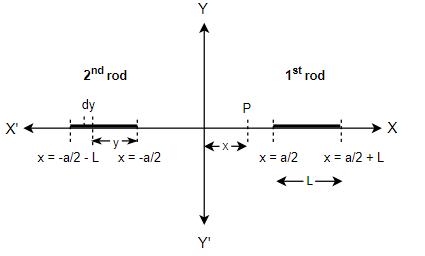
\includegraphics[scale = 0.75]{figures/Sandesh's Figures/2rd1.png}
    \caption{System of two rods placed on x-axis.}
    \label{2rd1}
\end{figure}
i. Consider a point P in positive x-axis at a distance x from the origin.\\
Consider a small segment dy of $2^{nd}$ rod at a distance y from its free end as shown in figure \ref{2rd1}.\\
Charge per unit length, ($\lambda$) = Q/L
\vspace{3pt}
\\
Charge within dy (dq) = (Q/L) $\cdot$ dy 
\vspace{3pt}
\\
Electric field at P due to dq, \[dE = \cfrac{1}{4 \pi \epsilon_o} \cdot \cfrac{{(Q/L)\cdot}dy}{\{y+ (a/2) + x\}^2}\]
Hence, the required electric field due to second rod at points along +ve x-axis,
\begin{align*}
       E &= \cfrac{Q}{4 \pi \epsilon_o L} \int_0^L \cfrac{dy}{{\{y+ (a/2) + x\}^2}}\\
         &= \cfrac{Q}{4 \pi \epsilon_o L} \int_0^L \{y+ (a/2) + x\}^{-2} dy\\
         &= \cfrac{Q}{4 \pi \epsilon_o L} \bigg[\cfrac{\{y+ (a/2) + x\}^{-2+1}}{-2+1}\bigg]_0^L\\
         &= -\cfrac{Q}{4 \pi \epsilon_o L} \bigg[\cfrac{1}{\{L+ (a/2) + x\}} - \cfrac{1}{x + (a/2)}\bigg ]\\
         &= \cfrac{Q}{2 \pi \epsilon_o L} \bigg[\cfrac{1}{2x+a} - \cfrac{1}{2x + a + 2L}\bigg ]
\end{align*}
ii. Let us consider a small segment dx on the first rod at a distance x from the origin.\\ 
Then, charge within dx (dq') = (Q/L)dx
\vspace{3pt}
\begin{figure}[h]
    \centering
    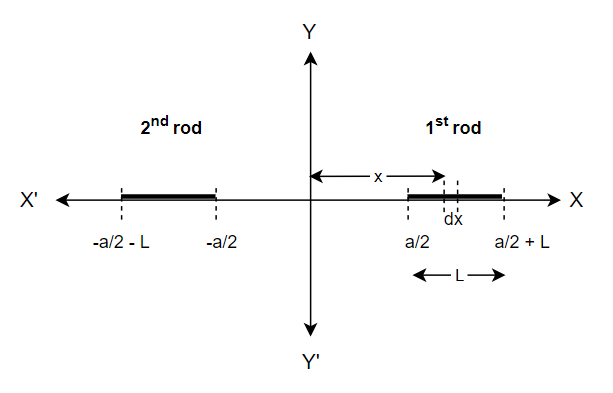
\includegraphics[scale = 0.58]{figures/Sandesh's Figures/2rd2.png}
    \caption{System of two rods placed on x-axis.}
    \label{2rd2}
\end{figure}
\\
The force on dq due to the second rod is given by,
\begin{align*}
    dF &= dq \cdot E\\
       &=\cfrac{Q}{L}\hspace{3pt} dx \cdot \cfrac{Q}{2 \pi \epsilon_o L} \bigg[\cfrac{1}{2x+a} - \cfrac{1}{2x + a + 2L}\bigg ]\\
        &=\cfrac{Q^2}{2 \pi \epsilon_o L^2} \bigg[\cfrac{dx}{2x+a} - \cfrac{dx}{2x + a + 2L}\bigg ]
\end{align*}
The total force exerted on the first rod, 
\begin{align*}
    F &= \cfrac{Q^2}{2 \pi \epsilon_o L^2} \bigg[\int_{a/2}^{(a/2)+L}\cfrac{dx}{2x+a} - \int_{a/2}^{(a/2)+L}\cfrac{dx}{2x + a + 2L}\bigg ]\\
      &= \cfrac{Q^2}{2 \pi \epsilon_o L^2} \bigg[\cfrac{1}{2} \bigg\{ln(a+2x)\bigg\}_{a/2}^{(a/2)+L} - \cfrac{1}{2} \bigg\{ln (2x + a + 2L)\bigg\}_{a/2}^{(a/2)+L}\bigg]\\
      &= \cfrac{Q^2}{4 \pi \epsilon_o L^2} \bigg[ln\cfrac{2a +2L}{2a} - ln\cfrac{2a + 4L}{2a + 2L}\bigg]\\
      &= \cfrac{Q^2}{4 \pi \epsilon_o L^2} \bigg[ln\cfrac{(a + L)^2}{a(a + 2L)} \bigg]
\end{align*}
iii. The reduced expression for force can be obtained as
\begin{align*}
    F &= \cfrac{Q^2}{4 \pi \epsilon_o L^2} \cdot ln\cfrac{\big[(a/a) + (L/a)\big]^2} {\big[(a^2/a^2) + (2aL/a^2)\big]} \\
      &= \cfrac{Q^2}{4 \pi \epsilon_o L^2} \cdot ln\cfrac{\big[1 + (L/a)\big]^2} {\big[(1 + (2L/a)\big]}\\
      &= \cfrac{Q^2}{4 \pi \epsilon_o L^2} \big[2 ln(1 + L/a) - ln (1 + 2L/a)\big] \\
      &= \cfrac{Q^2}{4 \pi \epsilon_o L^2} \bigg[\cfrac{2L}{a} - \cfrac{2L^2}{2a^2} - \cfrac{2L}{a} + \cfrac{4L^2}{2a^2} \bigg ] \hspace{10pt} [\because a\ll L]\\
      &= \cfrac{Q^2}{4 \pi \epsilon_o L^2} \cdot \cfrac{2L^2}{2a^2}\\
      &= \cfrac{Q}{4 \pi \epsilon_o a^2}
\end{align*}
This shows that if a $\ll$ L, then the two rods interact as point charges, which clearly makes sense.

\newpage
\begin{tcolorbox}
\textbf{9. An uncharged shell of radius a is surrounded by another concentric shell of radius b carrying a charge Q. Determine the potential of each shell. What will be the situation when inner shell is grounded? Observe the potential difference and capacitance.}
\end{tcolorbox}
Solution:\\
For a metallic shell of radius R and charge Q, potential on the surface and at any point inside is same and given by \[ V = \cfrac{1}{4 \pi \epsilon_o}\cdot \cfrac{Q}{R}\]
Any conducting object inside such shell will also be at same potential.\\
When a conducting body is connected to the earth its potential becomes zero.
\begin{figure}[h]
    \centering
    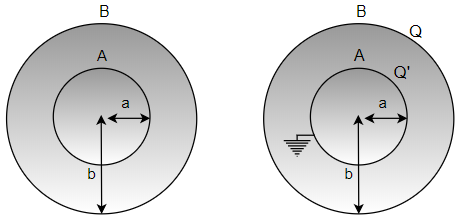
\includegraphics[scale = 0.6]{figures/Sandesh's Figures/bag.png}
    \caption{Before and after grounding the inner shell.}
    \label{bag}
\end{figure}
\\
\textbf{\underline{Before grounding inner shell}}
\vspace{3pt}
\\
As there is no charge in the inner shell, potential is due to charge on outer shell only. \\
Potential on the outer shell $(V_B) = \cfrac{1}{4 \pi \epsilon_o}\cdot \cfrac{Q}{b}$\\
From above discussion,\\
Potential on the inner shell $(V_A) = \cfrac{1}{4 \pi \epsilon_o}\cdot \cfrac{Q}{b}$
\vspace{3pt}
\\
This shows that there is no any potential difference between shell A and shell B.\\
 \textbf{\underline{After grounding inner shell}}
\vspace{3pt}
\\
After grounding the inner shell, charges (electrons) flow from earth (zero potential) to inner shell (higher potential) and the potential of inner shell becomes zero. Let Q' be the amount of charge developed on inner shell. \\
The potential due to Q' $(V_A') =  \cfrac{1}{4 \pi \epsilon_o}\cdot \cfrac{Q'}{a}$\\
Here $V_A$ and $V_A'$ should combine to give zero potential.
\begin{align*}
   V_A + V_A' &= 0
    \text{or, } \cfrac{1}{4 \pi \epsilon_o}\cdot \cfrac{Q'}{a} &= - \cfrac{1}{4 \pi \epsilon_o}\cdot \cfrac{Q}{b} 
   \therefore Q' &= -\cfrac{a}{b} Q
\end{align*}

   This is the amount of charge induced on the inner shell. Because of this charge at A, the potential at B will also change. \\
   Potential of B after grounding,\\
   ($V_B'$) = Potential due to Q on shell B + Potential due to Q' on shell A
   \[\therefore V_B' = \cfrac{1}{4 \pi \epsilon_o}\cdot \cfrac{Q}{b} + \cfrac{1}{4 \pi \epsilon_o}\cdot \cfrac{Q'}{b} \]
   Putting  $Q' = -\cfrac{a}{b} Q$ we get,
   \[ V_B' = \cfrac{Q}{4 \pi \epsilon_o}\cdot \cfrac{b -a}{b^2} \]
Potential difference between the shells (P.D) $= V_B' - 0 = V_B$
\vspace{3pt}
\\
The capacitance of the system (C) = $\cfrac{Q}{P.D} = \cfrac{Q}{\cfrac{Q (b - a)}{4 \pi \epsilon_o b^2}} = \cfrac{4 \pi \epsilon_o b^2}{b - a}$






\newpage
\section{Practice Problems}
\begin{enumerate}
   \item A soap bubble of radius r and surface tension T is given a potential V volts. Show that the radius R of the bubble is related to its initial radius by the equation
\[ P(R^3 - r^3) + 4T(R^2 - r^2) - \cfrac{\epsilon_oV^2R}{2} = 0,\]
where P is the atmospheric pressure.

\item A sphere of uniform density $\rho$ has within it a spherical cavity whose centers is at a distance a from the sphere. Show that the gravitational field within the cavity is uniform and determine its magnitude. \big(Ans : -4/3 $\pi$G$\rho$a\big)

\item An atom can be approximately treated as consisting of a uniform spherical electron density (electron cloud) of radius R with total charge -Ze and positive charge nucleus +Ze at the center, where e is the charge of a positron. The nucleus mass is much larger than an electron mass m$_e$. In a uniform external electric field E$_o$ the electron cloud is displaced slightly from the nucleus while maintaining its spherical shape. Find the displacement. 

\begin{figure}[htp]
    \centering 
    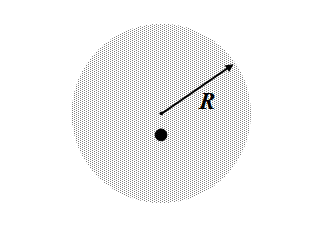
\includegraphics{mainmatter/electro1.PNG}
    \caption{}
    \label{fig:my_label}
\end{figure}
\item Two point charges q and 2q are fixed on a smooth horizontal rail separated by a distance L. A small cart carrying charge q and with mass m can move freely on the rail, as shown in the figure. Find the simple harmonic oscillation frequency of the cart. 
\begin{figure}[htp]
    \centering 
    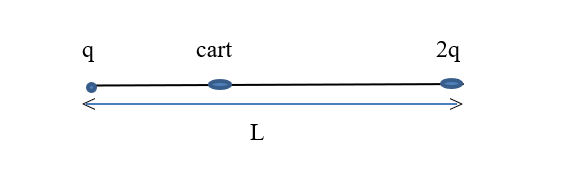
\includegraphics{mainmatter/electro2.PNG}
    \caption{}
    \label{fig:my_label}
\end{figure}
\item A spatially uniform magnetic field B~ exists in the circular region S and this field is decreasing in
magnitude with time at a constant rate (see Fig. (1)). The wooden ring C$_1$ and the conducting ring C$_2$ are concentric with the magnetic field. The magnetic field is perpendicular to the plane
of the figure. Then
\begin{enumerate}
    \item there is no induced electric field in C$_1$.
    \item there is an induced electric field in C$_1$ and its magnitude is greater than the magnitude of the induced electric field in C$_2$.
    \item there is an induced electric field in C$_2$ and its magnitude is greater than the induced electric field in C$_1$.
    \item there is no induced electric field in $C_2$. 
\end{enumerate}
\hfill \textsl{(InPhO)}\\
\textbf{Ans:} (b)

\item A non-conducting sphere having a spherical cavity centered at a distance \textbf{a} from the center of the sphere. Charge on the sphere is distributed uniformly with volume density $\rho$. A particle of mass \textbf{m} having charge -\textbf{q} is suspended vertically from the light non-conducting spring of force constant \textit{k}. Find time period and acceleration? (No gravity and initially when -q is suspended spring was of natural length.) 
\hfill \textsl{(IIT JEE)} \\
\textbf{Answer:} Time period(T) = $2\pi \sqrt{\dfrac{m}{k}}$; acceleration = $\dfrac{q}{m}$$\dfrac{\rho a}{3 \epsilon_o}$
\end{enumerate}
